Fig. \ref{fig:siso-channels} illustrates the frequency response of a SISO FF and FS channel based on the same tap delays and tap gains.

\begin{figure}[ht]
  \centering
  \subfigure[FF channel]{
    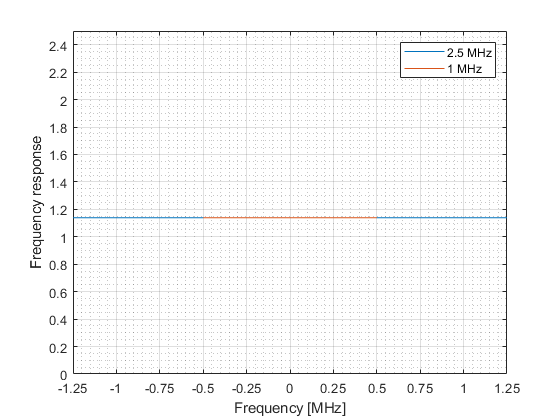
\includegraphics[width=0.48\textwidth]{siso_frequency_flat_channel}\label{fig:siso-ff}}
  \subfigure[FS channel]{
    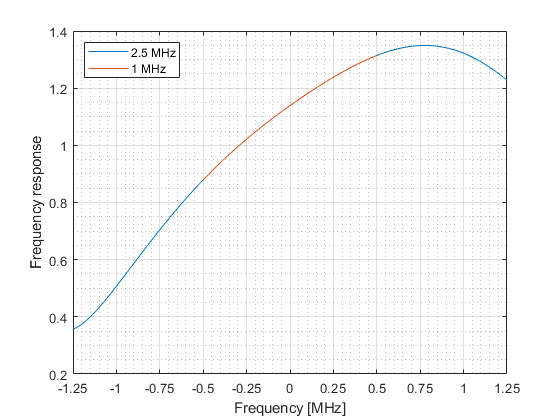
\includegraphics[width=0.48\textwidth]{siso_frequency_selective_channel}\label{fig:siso-fs}}
  \caption{Frequency response of the SISO FF and FS channels}\label{fig:siso-channels}
\end{figure}

In the R-E plots, the rightmost point of each curve indicates the maximum achievable rate with zero harvested DC current. It corresponds to WIT that allocates all available power to the modulated information waveform by the water-filling algorithm with $\rho  = 0$. Note that the x-axis here refers to the per-subband rate and is normalized w.r.t. bandwidth. With a fixed power budget, the power received by each subband decreases as $N$ increases. Therefore, the rate achieved by each subband decreases but the total rate increases. On the other hand, the leftmost point corresponds to the maximum output DC current with zero information rate, which correspond to allocating all power to the multisine waveform with $\rho  = 1$ (WPT).

Nevertheless, the discrete rate constraint \eqref{eqn:original_rate_constraint} in the optimization problem prevent the solutions from achieving the absolute WIT points using the proposed WIPT approach. Therefore, we perform an individual WIT and combine the results for closed R-E plots.

\subsection{R-E Region vs Subband}\label{sec:re-region-vs-subband}
Fig. \ref{fig:siso-subband} illustrates the R-E region against subband $N = 1,2,4,8,16$ for superposed waveform and no power waveform over FF and FS channels respectively.

\begin{figure}[ht]
  \centering
  \subfigure[FF: Superposed waveform]{
    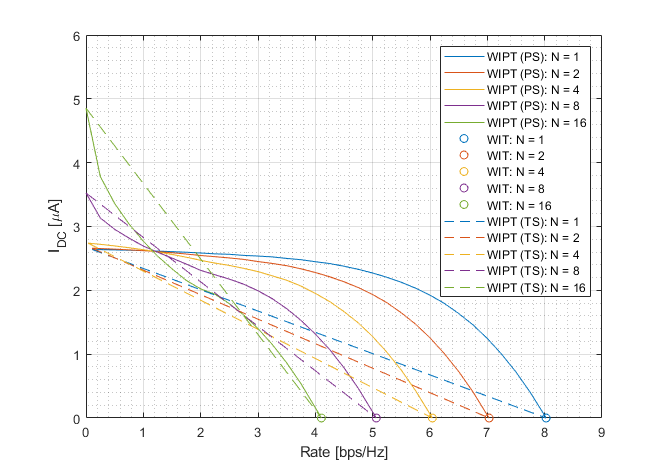
\includegraphics[width=0.48\textwidth]{siso_re_ff_subband_superposed_waveform}\label{fig:subband-ff-superposed}}
  \subfigure[FF: No power waveform]{
    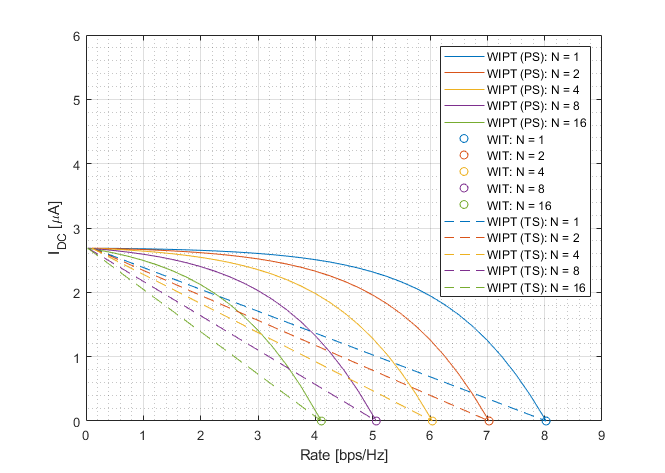
\includegraphics[width=0.48\textwidth]{siso_re_ff_subband_no_power_waveform}\label{fig:subband-ff-no-power}}
  \quad
  \subfigure[FS: Superposed waveform]{
    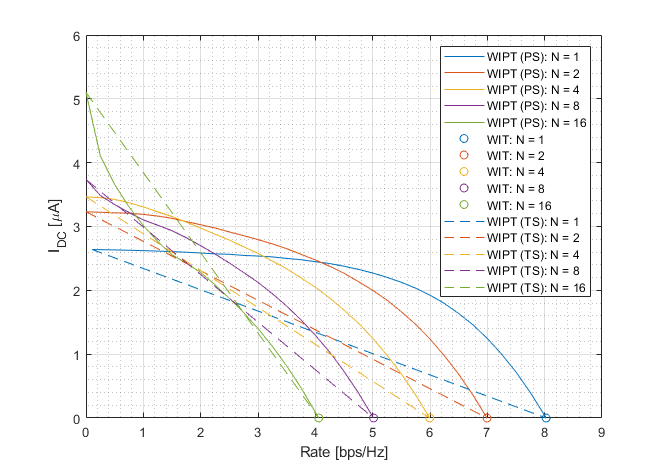
\includegraphics[width=0.48\textwidth]{siso_re_fs_subband_superposed_waveform}\label{fig:subband-fs-superposed}}
  \subfigure[FS: No power waveform]{
    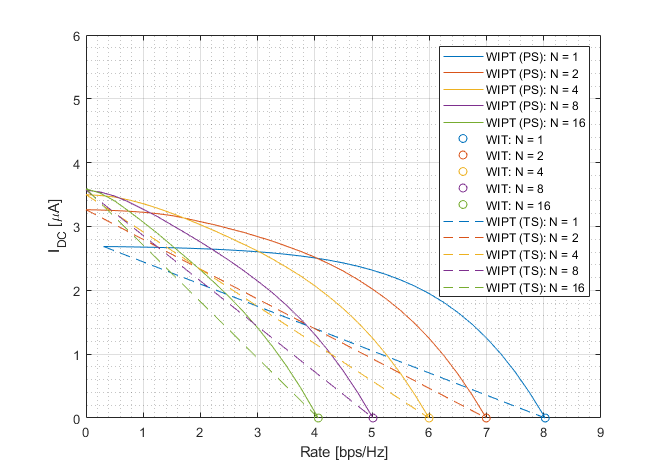
\includegraphics[width=0.48\textwidth]{siso_re_fs_subband_no_power_waveform}\label{fig:subband-fs-no-power}}
  \caption{R-E region vs $N$ for FF and FS channels}\label{fig:siso-subband}
\end{figure}

It can be observed that the introduction of multisine power waveform boosts the harvested energy for $N > 4$ where the superposed waveform outperforms the modulated signal for WIPT. In contrast, the R-E performance of both signals are very close for $N \leqslant 4$ so that multisine is unnecessary. The reason is that the fourth order terms of power and information waveforms \eqref{eqn:power_waveform_fourth_order} and \eqref{eqn:information_waveform_fourth_order} have different contribution to the harvested DC current. Despite both posynomials consist of monomials of similar magnitude (${\prod\nolimits_{j = 0}^3 {{s_{P,{n_j},{m_j}}}{A_{{n_j},{m_j}}}} }$ and $\prod\nolimits_{j = 0,2} {{s_{I,{n_0},{m_j}}}{A_{{n_0},{m_j}}}} \prod\nolimits_{j = 1,3} {{s_{I,{n_1},{m_j}}}{A_{{n_1},{m_j}}}} $ ), the power posynomial contains $(2{N^3} + N)/3$ monomials but the information posynomial only holds ${N^2}$ monomials. Therefore, the energy benefit of multisine is amplified with a large $N$. Although it seems that a very large $N$ can significantly increases the output DC current, this is not true because each subband will receive less power such that the amplitude of monomials decreases accordingly.

A contrast of R-E plots on FF and FS channels also indicates the benefit of frequency selectivity on the harvested power. The gain is particularly obvious in the low-rate region, where all the power is allocated to the subband with the strongest amplitude. We observe from the FS channel instance in Fig. \ref{fig:siso-fs} that some edge frequencies enjoy a larger gain than the center frequency, whose advantage is exploited when more subbands are used. In comparison, the small amplitude at the center frequency accounts for the lower output DC current when $N = 1$ (indicated by the blue curves in Fig. \ref{fig:subband-fs-superposed} and \ref{fig:subband-fs-no-power}).

Without power waveform, the R-E region appears convex such that PS dominates TS over all $N$. On the other hand, the R-E region achieved by superposed waveform with PS is convex for $N = 2,4$ but concave-convex for $N = 8,16$. Therefore, the optimal strategy is using PS for small $N$, TS for large $N$, and a combination of PS and TS for medium $N$. As shown in Fig. \ref{fig:siso-subband-optimal}, the best curve for medium $N$ consists of two parts. The straight part is achieved by TS between WPT (multisine only with $\rho  = 1$) that corresponds to the leftmost point and WIPT (superposed waveform with $0 < \rho  < 1$) that corresponds to the tangent point, while the convex part is the contribution of WIPT only. The characteristics of the optimal R-E region comes from the rectifier nonlinearity.

\begin{figure}[ht]
  \centering
  \subfigure[Optimal strategy for $N = 8$]{
    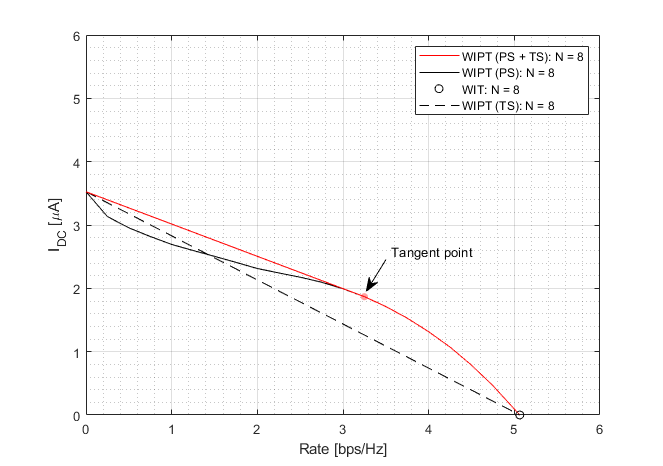
\includegraphics[width=0.48\textwidth]{siso_re_ff_subband_8_optimal}\label{fig:subband-8-optimal}}
  \subfigure[Optimal strategy for $N = 16$]{
    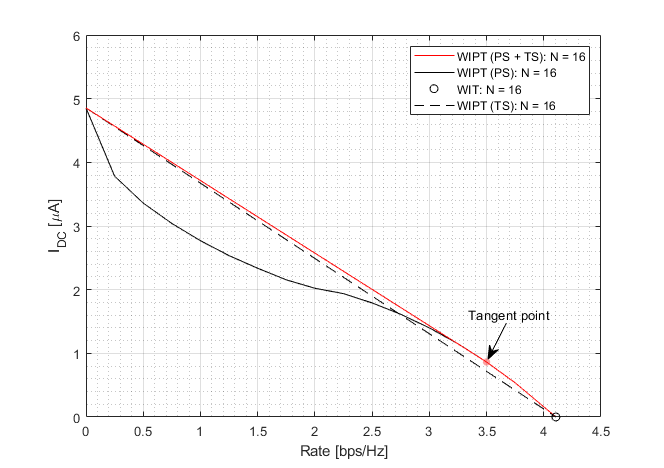
\includegraphics[width=0.48\textwidth]{siso_re_ff_subband_16_optimal}\label{fig:subband-16-optimal}}
  \caption{Optimal R-E region for FF channel with medium $N$}\label{fig:siso-subband-optimal}
\end{figure}

Moreover, the plots over the FS channel suggests that for single-carrier transmission, the modulated waveform outperforms the superposed waveform for WPT. At a zero-approaching rate, the modulated waveform produces a DC current of \SI{2.69}{\uA} while the superposed waveform only delivers \SI{2.64}{\uA}. The actual current gap is even larger since the former still guarantees a slightly higher rate. On the contrary, the superposed waveform leads to a larger harvested current for $N \geqslant 2$. It demonstrates that modulation is beneficial in single-carrier transmission but can be detrimental in multi-carrier transmission. The reason is that the modulation gain \eqref{eqn:modulation_gain} of modulated waveform outperforms the energy benefit of multisine in single-carrier transmission but is outperformed in multi-carrier transmission. The result is inline with the scaling laws proposed in \cite{Clerckx2018}.

One problem is that the leftmost point of some curves did not start from the y-axis. Although a zero rate constraint is employed in WIPT, a candidate solution may achieve a nonzero rate. It is because the current gain of the next iteration is smaller than the threshold $\varepsilon$ so that the algorithm terminates and outputs the existing R-E pair. This phenomenon occurs primarily for small $N$ that produces a smaller current gain in each iteration and at the low-rate region where the output DC current almost saturated. It can be fixed either by reducing the threshold $\varepsilon$ or developing an individual function for WPT.



\subsection{R-E Region vs SNR}\label{sec:re-region-vs-snr}
Fig. \ref{fig:siso-ff-snr} and \ref{fig:siso-fs-snr} contrast the performance of the modulated waveform, ideal superposed waveform and its lower bound for $N = 16$ and ${\text{SNR}} = 10,20,30,40$ dB over the example FF and FS channels.

\begin{figure}[ht]
  \centering
  \subfigure[FF: ${\text{SNR}} = 10$ dB]{
    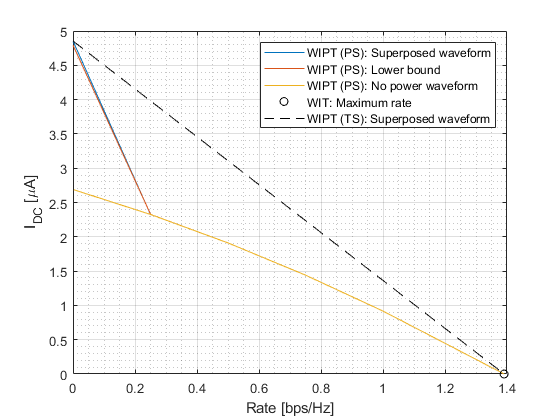
\includegraphics[width=0.48\textwidth]{siso_re_ff_snr_10dB}\label{fig:snr-ff-10db}}
  \subfigure[FF: ${\text{SNR}} = 20$ dB]{
    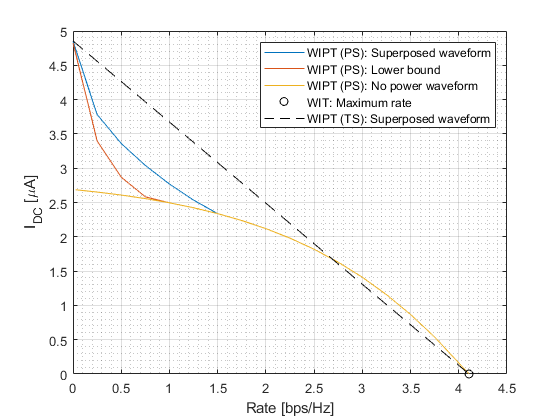
\includegraphics[width=0.48\textwidth]{siso_re_ff_snr_20dB}\label{fig:snr-ff-20db}}
  \quad
  \subfigure[FF: ${\text{SNR}} = 30$ dB]{
    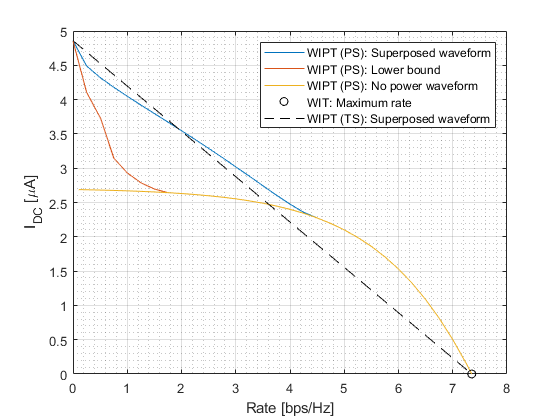
\includegraphics[width=0.48\textwidth]{siso_re_ff_snr_30dB}\label{fig:snr-ff-30db}}
  \subfigure[FF: ${\text{SNR}} = 40$ dB]{
    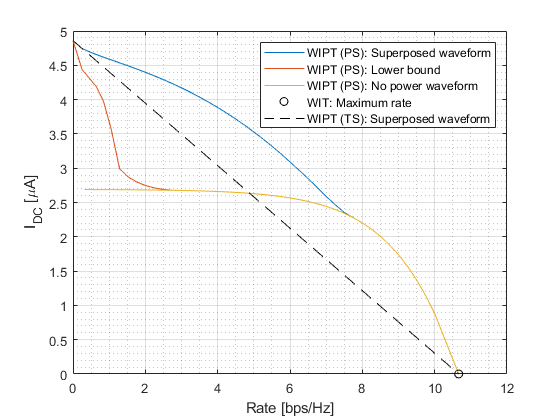
\includegraphics[width=0.48\textwidth]{siso_re_ff_snr_40dB}\label{fig:snr-ff-40db}}
  \caption{R-E region vs SNR for FF channel}\label{fig:siso-ff-snr}
\end{figure}

\begin{figure}[ht]
  \centering
  \subfigure[FS: ${\text{SNR}} = 10$ dB]{
    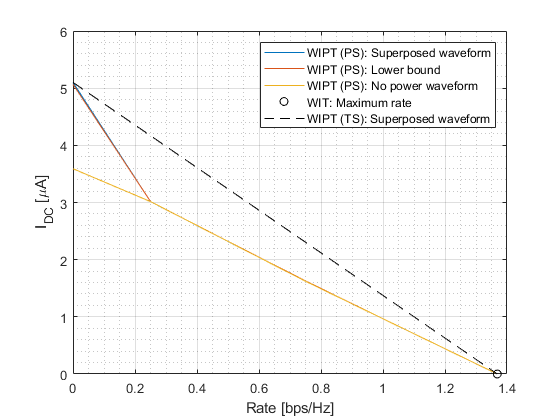
\includegraphics[width=0.48\textwidth]{siso_re_fs_snr_10dB}\label{fig:snr-fs-10db}}
  \subfigure[FS: ${\text{SNR}} = 20$ dB]{
    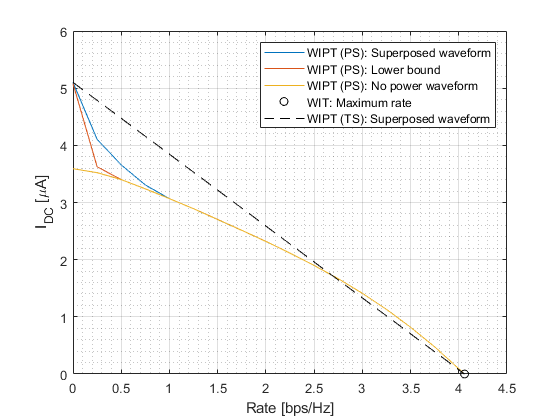
\includegraphics[width=0.48\textwidth]{siso_re_fs_snr_20dB}\label{fig:snr-fs-20db}}
  \quad
  \subfigure[FS: ${\text{SNR}} = 30$ dB]{
    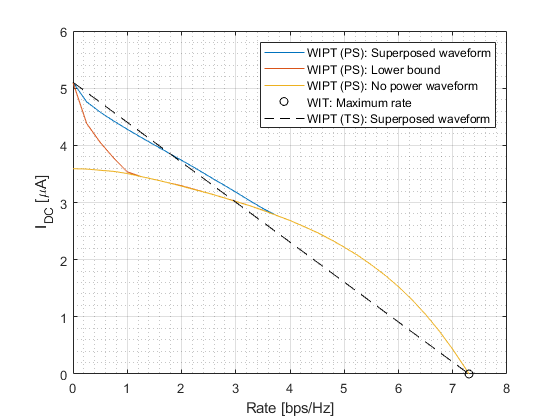
\includegraphics[width=0.48\textwidth]{siso_re_fs_snr_30dB}\label{fig:snr-fs-30db}}
  \subfigure[FS: ${\text{SNR}} = 40$ dB]{
    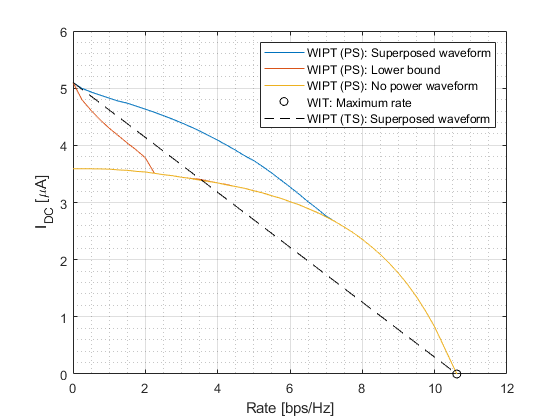
\includegraphics[width=0.48\textwidth]{siso_re_fs_snr_40dB}\label{fig:snr-fs-40db}}
  \caption{R-E region vs SNR for FS channel}\label{fig:siso-fs-snr}
\end{figure}

Thanks to the contribution of multisine waveform, the R-E region of the superposed signal is enlarged in both cases. This phenomenon is especially obvious in the low-rate region, where the multisine dominates the transmission. It results from the fact that the nonlinear rectifier favors the deterministic multisine with high PAPR. On the contrary, there is some randomness involved in the modulated waveform that produces fluctuations to the rectifier and leads to some power loss \cite{Clerckx2018}. This phenomenon is in sharp contrast to the conclusion based on linear harvester model that both waveforms are equally suitable for WPT \cite{Xu2014a}. As shown in the plots, even with the assumption that the deterministic power waveform creates some interference to the information waveform, the rate loss is compensated by the power gain such that the superposed waveform strictly outperforms the modulated waveform.

Another observation is the performance gap between the ideal superposed waveform and its lower bound widens as SNR increases. This is as expected because the rate is dominated by noise at low SNR and by interference at high SNR. For ${\text{SNR}} = 10$ dB, the interference is much lower than noise even if a large amount of power is allocated to the multisine component. Hence, the curves almost overlap with each other. On the other hand, at a higher SNR, the rate loss by interference increases while the energy benefit of power waveform remains unchanged. To obtain the optimal R-E tradeoff, the transmitter tends to allocate less power to the multisine so that the harvested current drops. Therefore, the rate boost of deterministic power waveform grows as SNR increases.

The plots also demonstrate that for the superposed waveform with a sufficiently large $N$, TS is preferred at low SNR and PS is favored at high SNR, while a combination of TS and PS is generally optimal for medium SNR. On the other hand, the R-E region is strictly convex for the modulated waveform-only transmission due to its inefficiency to boost the harvested energy. It corresponds to the conventional opinion that PS always outperforms TS for no power waveform transmission. In this case, the R-E curve is approximately straight at low SNR but with large curvature at high SNR. The reason is that at a low SNR, the water-filling strategy concentrates the power to the best subband to maximize the rate, and the region boundary is obtained by varying $\rho $ only. In comparison, more subbands are utilized in the transmission as SNR increases. Therefore, only a small portion of power is required to achieve a decent rate while the remaining part can be used to boost the output current.

A comparison between the results over FF and FS channels emphasizes the benefit of frequency selectivity on the harvested current. The gain is more significant for modulated waveform (around \SI{1}{\uA}) than superposed waveform (around \SI{0.25}{\uA}). One possible reason is that the power are concentrated in few subbands such that the number of terms in \eqref{eqn:power_waveform_fourth_order} and \eqref{eqn:information_waveform_fourth_order} are comparable. In such cases, the impact of channel amplitude on each monomial is more significant on the information waveform and contributes to a larger gain in the harvested current.



\subsection{R-E Region vs PAPR}\label{sec:re-region-vs-papr}
Fig. \ref{fig:re-papr} investigates the relationship between PAPR and R-E region for $N = 8, 16$ over the FF and FS channels.

\begin{figure}[ht]
  \centering
  \subfigure[FF: $N = 8$]{
    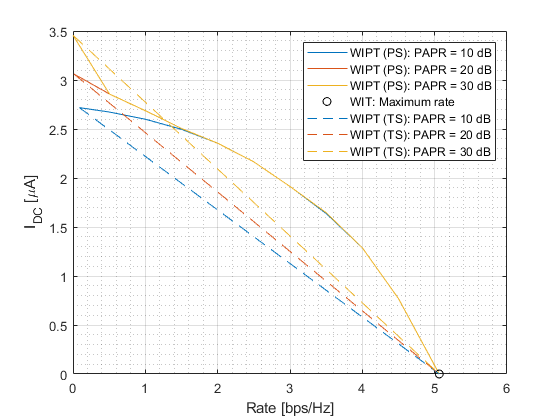
\includegraphics[width=0.48\textwidth]{siso_re_ff_papr_8}\label{fig:re-ff-papr-8}}
  \subfigure[FF: $N = 16$]{
    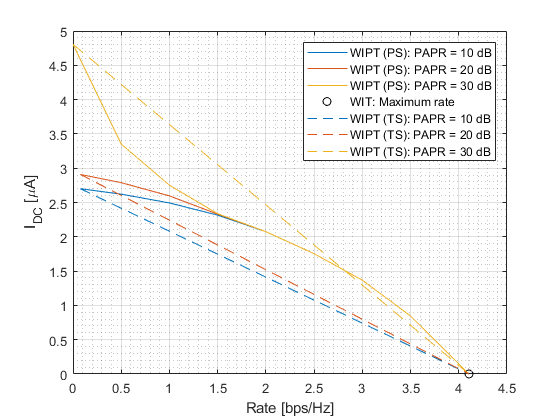
\includegraphics[width=0.48\textwidth]{siso_re_ff_papr_16}\label{fig:re-ff-papr-16}}
  \quad
  \subfigure[FS: $N = 8$]{
    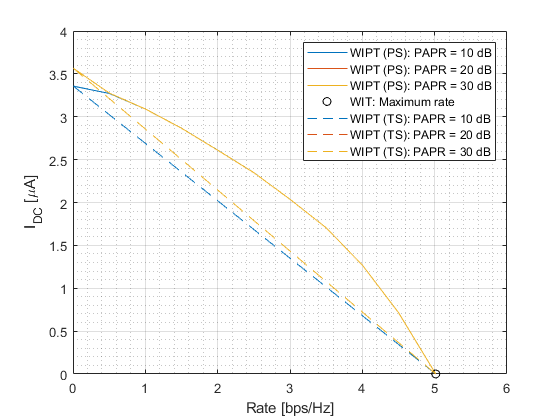
\includegraphics[width=0.48\textwidth]{siso_re_fs_papr_8}\label{fig:re-fs-papr-8}}
  \subfigure[FS: $N = 16$]{
    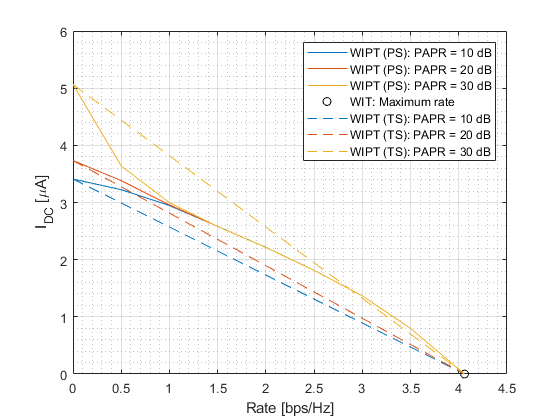
\includegraphics[width=0.48\textwidth]{siso_re_fs_papr_16}\label{fig:re-fs-papr-16}}
  \caption{R-E region vs PAPR for FF channel}
  \label{fig:re-papr}
\end{figure}

A first observation is that a large enough PAPR is required to fully exploit the power gain of the multisine waveform. For $N = 16$, the R-E region is convex for a PAPR no larger than 20 dB and is concave-convex when it increases to 30 dB. For instance, with a small PAPR of 10 dB, the use of multisine waveform is strictly constrained such that the modulated waveform dominates the transmit signal. Hence, the corresponding R-E plot is similar to the result without power waveform. On the contrary, a PAPR of 30 dB is large enough to achieve the optimal performance of the superposed signal in the low-rate region. It can be concluded that the energy benefit of the multisine waveform indeed comes from the high PAPR. In each cycle, the peak pushes the rectifier output voltage to a high level which decreases slowly in the rest of the period.

A contrast of the R-E plots of $N = 8$ and 16 also suggests a larger $N$ requires higher PAPR to improve the performance. When PAPR increases from 20 to 30 dB, the current gain is more significant for $N = 16$ than $N = 8$. On the other hand, the impact of PAPR for small $N$ is not as significant as for large $N$. This verifies the positive correlation between $N$ and PAPR discussed in Section \ref{sec:rectifier-behavior}. Although increasing $N$ in a proper range can effectively boost the harvested energy, the PAPR constraint may limit the use of a large $N$ in practice.

It is interesting to notice that the frequency selectivity helps to achieve the optimal R-E region with a lower PAPR. As shown in Fig. \ref{fig:re-fs-papr-8}, a PAPR constraint of 20 dB is enough to guarantee the best tradeoff and a larger budget is unnecessary. However, the transmission over the FF channel requires a larger PAPR of 30 dB to achieve optimum behavior. This is because frequency selective channel can further amplify the difference of frequency components such that the received signal is with enhanced PAPR. 

The main disadvantage of the proposed approach is that the oversampling procedure further increases the overall computational complexity in the optimization. 